\documentclass[12pt,letterpaper]{article}
\usepackage[utf8]{inputenc}
\usepackage[T1]{fontenc}
\usepackage{lmodern}
\usepackage{graphicx}
\usepackage{caption}
\captionsetup{
    font=small,
    labelfont=bf,
    textfont=md,
    format=hang,
    justification=centering,
    textformat=period,
}
\usepackage{float}
\usepackage{geometry}
\usepackage{microtype}
\usepackage[breaklinks=true,hidelinks]{hyperref}
\usepackage{listings}
\usepackage{xcolor}
\usepackage[most]{tcolorbox}
\usepackage{amsmath}
\usepackage{cleveref}
\usepackage{textcomp}
 \newcommand{\mytexttilde}{\raisebox{0.5ex}{\texttildelow}}
% Set page margins
% \geometry{
%     a4paper,
%     left=25mm,
%     right=25mm,
%     top=25mm,
%     bottom=25mm,
% }

% Define custom style for listings
\lstdefinestyle{custombash}{
    language=bash,
    basicstyle=\ttfamily\small,
    keywordstyle=\color{blue},
    commentstyle=\color{gray},
    stringstyle=\color{red},
    backgroundcolor=\color{gray!10},
    frame=single,
    breaklines=true,
    showstringspaces=false,
}

\begin{document}

\title{\LARGE SSH Key Generation, Adding to SSH Agent, and Uploading to the Cluster}
\author{Markus G. S. Weiss}
\date{2024/10/28}
\maketitle

\tableofcontents
\newpage
\section{Introduction}

This guide will walk you through generating SSH keys, adding your private key to an SSH agent, and uploading your public key to the cluster for secure authentication. Instructions are provided for both Windows and macOS/Linux users.

\section{Generating SSH Keys}

SSH keys are used for secure authentication between your local machine and the server. Follow the steps below based on your operating system.

\subsection{Installing OpenSSH Client (Windows Only)}

\begin{enumerate}
    \item If you are using \textbf{Windows} (11), ensure that the OpenSSH Client is enabled on your machine.
    \begin{enumerate}
        \item Open \textbf{Settings} and search for \textbf{Optional features} or navigate to \textbf{System} $\rightarrow$ \textbf{Optional features} for Windows 11 or \textbf{Apps} $\rightarrow$ \textbf{Apps and Features} $\rightarrow$ \textbf{Manage Optional Features} for other versions.
        \item Search for \textbf{OpenSSH Client}. If not found, proceed with the next steps.
        \item Click on \textbf{Add a feature}.
        \item Search for \textbf{OpenSSH Client} and install it.
    \end{enumerate}

    \begin{figure}[H]
        \centering
        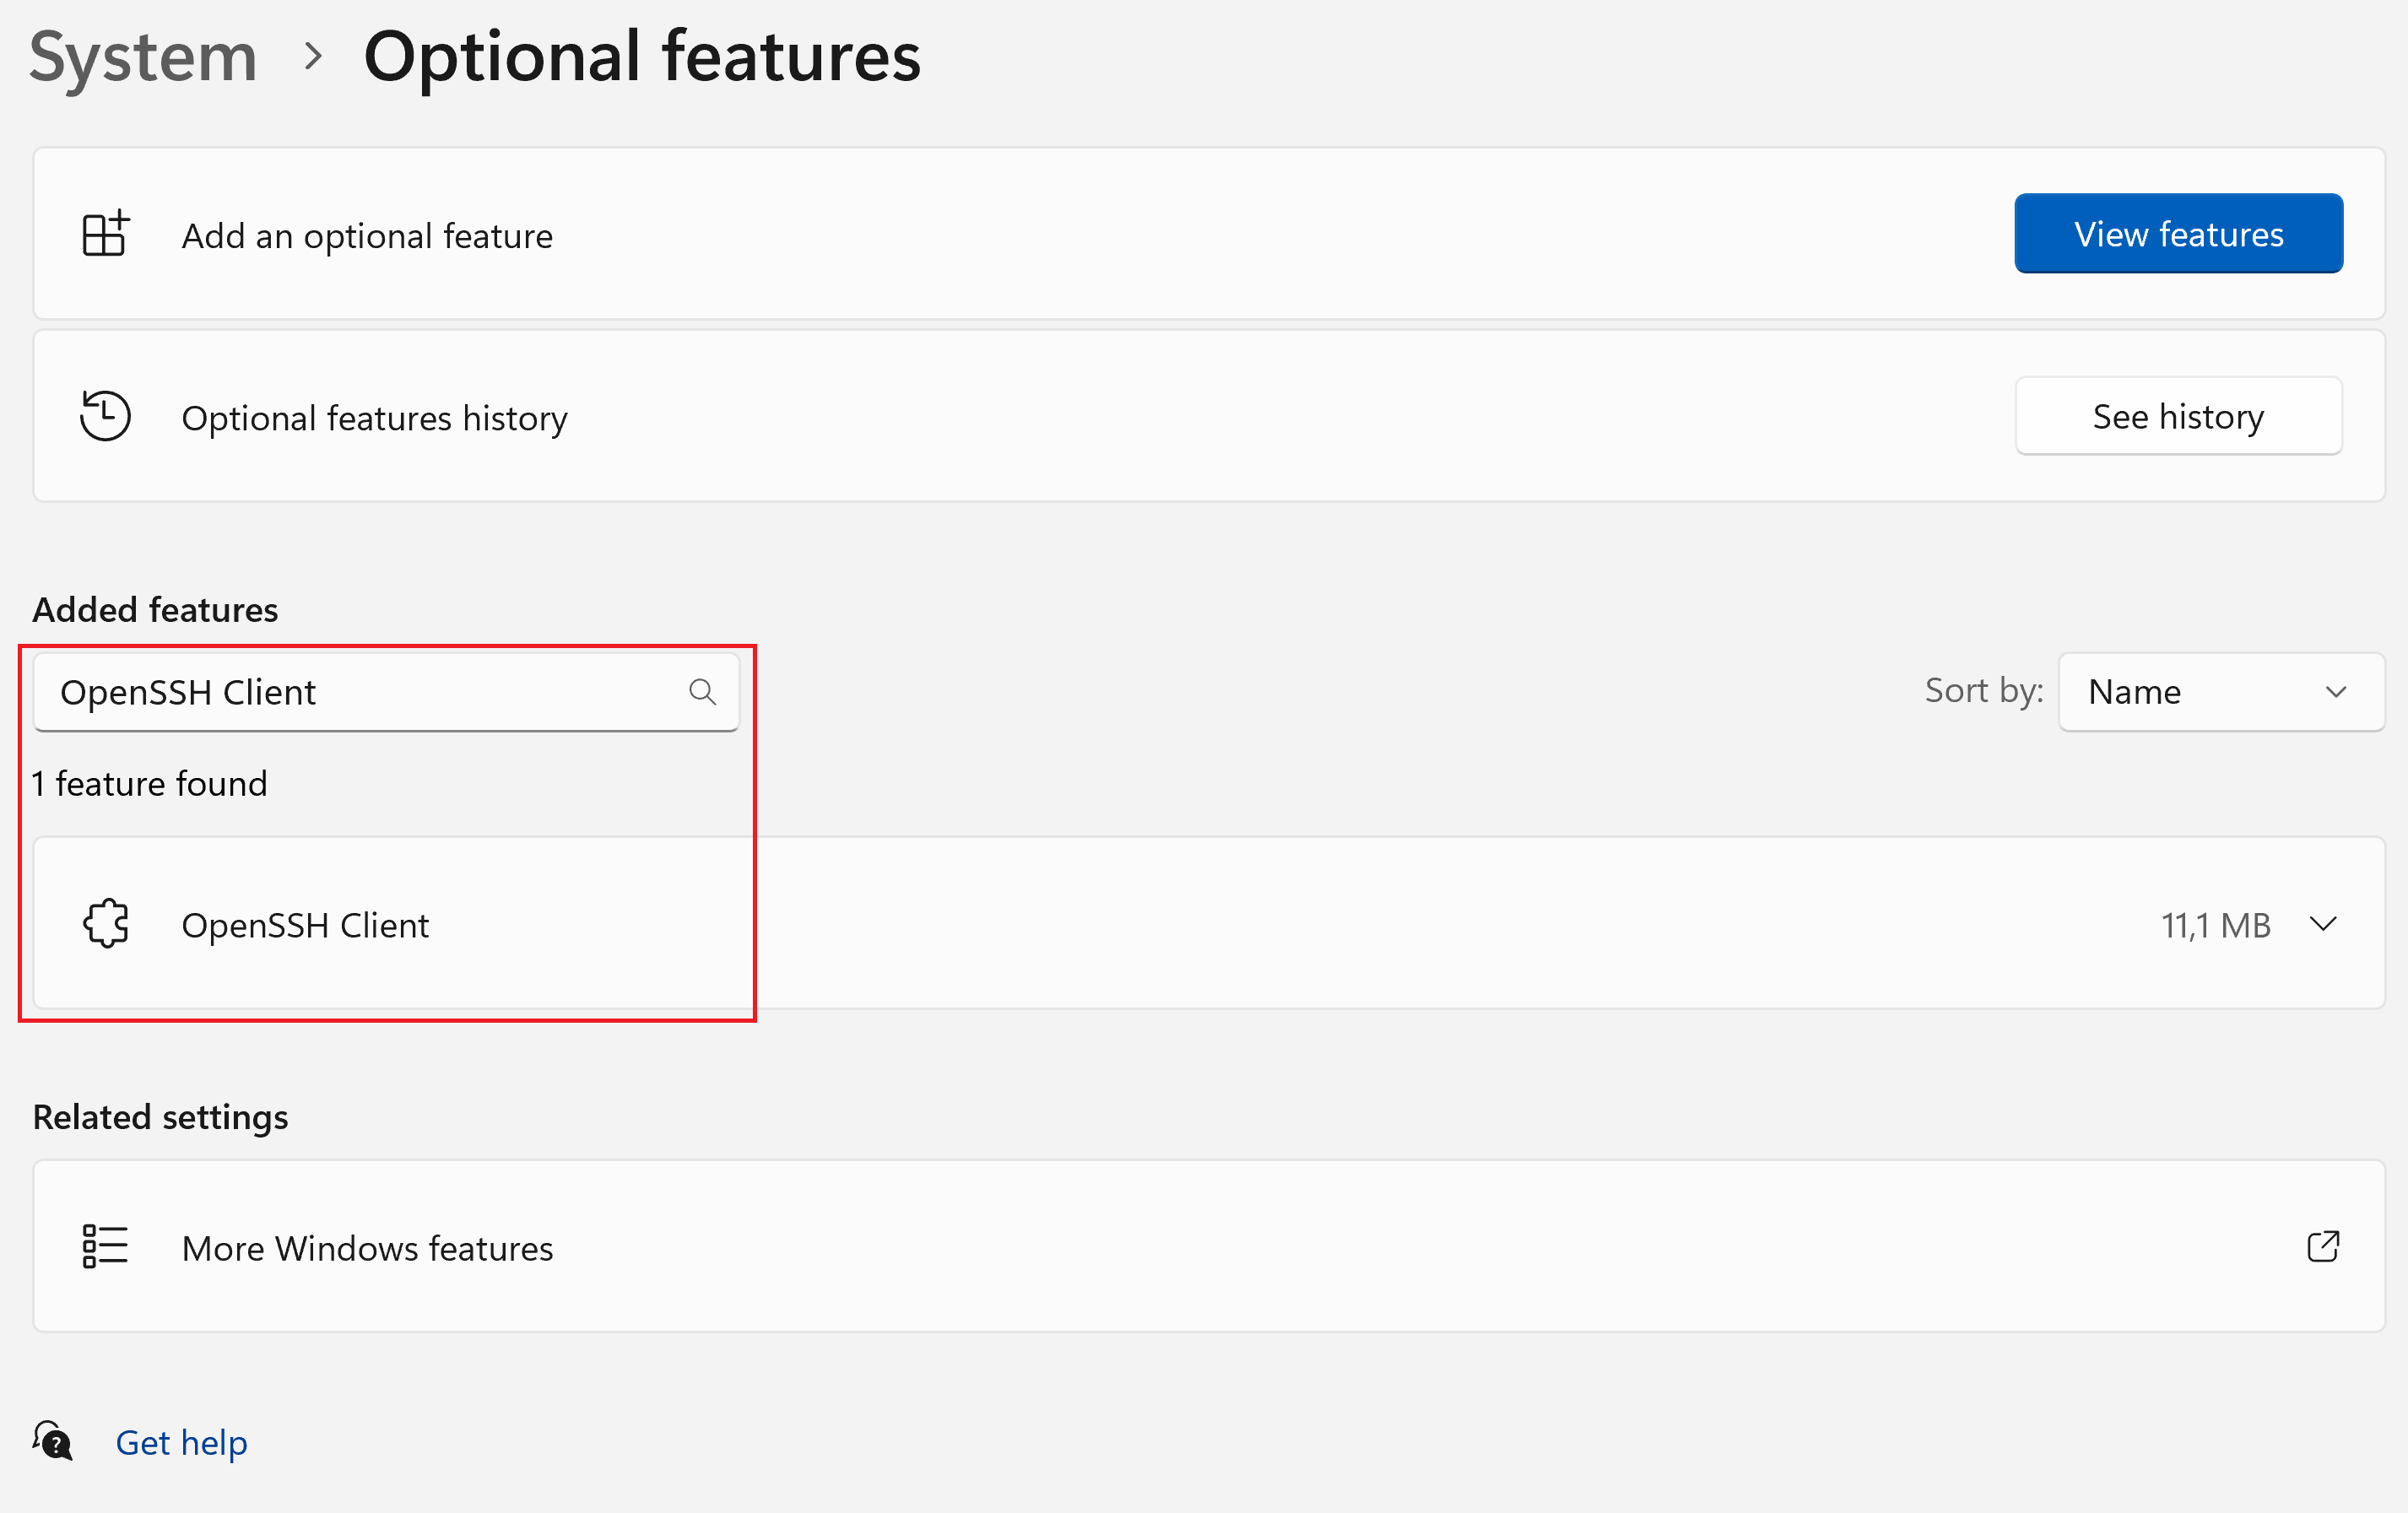
\includegraphics[width=0.7\textwidth]{openssh_client.png}
        \caption{Enabling the OpenSSH Client in Windows Settings}
        \label{fig:openssh_client}
    \end{figure}
\end{enumerate}

\subsection{Opening the Terminal}

\begin{enumerate}
    \item Open the appropriate terminal for your operating system:
    \begin{itemize}
        \item \textbf{Windows Users}: Open \textbf{Command Prompt} (Press \textbf{Windows key + R}, type \texttt{cmd}, and click \textbf{OK}).
        \item \textbf{macOS/Linux Users}: Open \textbf{Terminal} (macOS: Press \textbf{Command + Space}, type \texttt{Terminal}, and press \textbf{Enter}; Linux: Press \textbf{Ctrl + Alt + T} or search for \texttt{Terminal}).
    \end{itemize}

    \begin{figure}[H]
        \centering
        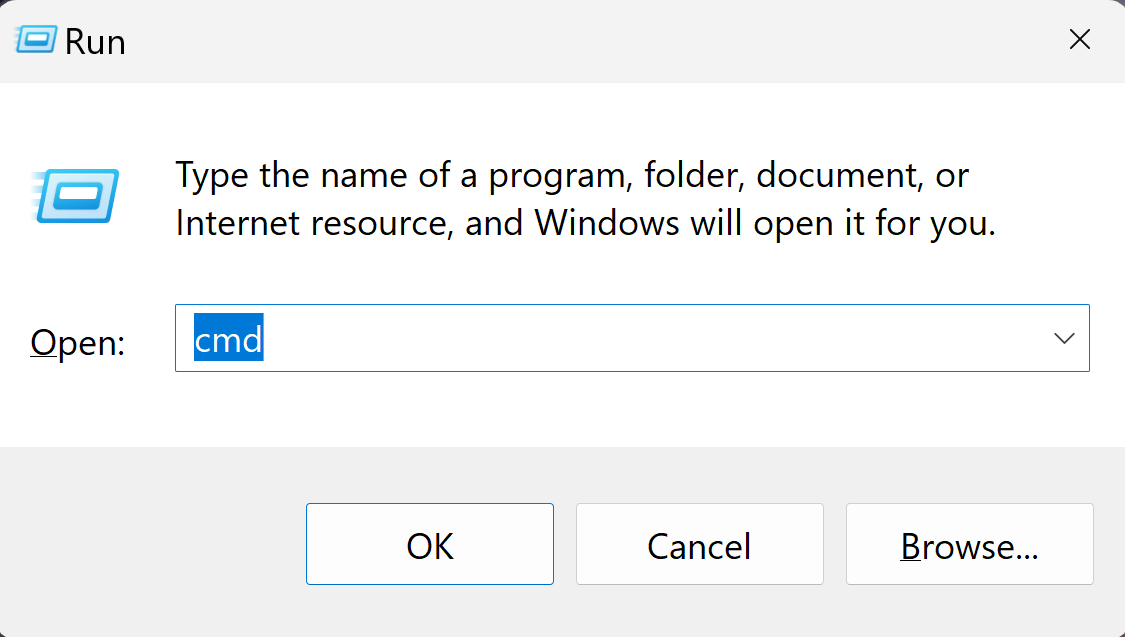
\includegraphics[width=0.7\textwidth]{command_prompt.png}
        \caption{Opening Command Prompt}
        \label{fig:command_prompt}
    \end{figure}
\end{enumerate}

\subsection{Checking for Existing SSH Keys}

Before generating a new SSH key, check if you already have one.

\begin{enumerate}
    \setcounter{enumi}{1}
    \item List the contents of the \texttt{\mytexttilde/.ssh} directory:
    \begin{itemize}
        \item \textbf{Windows}:
        \begin{lstlisting}[style=custombash]
dir %USERPROFILE%\.ssh
        \end{lstlisting}
        \item \textbf{macOS/Linux}:
        \begin{lstlisting}[style=custombash]
ls ~/.ssh
        \end{lstlisting}
    \end{itemize}
    \item If you see files like \texttt{id\_ed25519} and \texttt{id\_ed25519.pub}, you already have an SSH key pair. You can use these existing keys or generate a new pair if necessary.

    \begin{figure}[H]
        \centering
        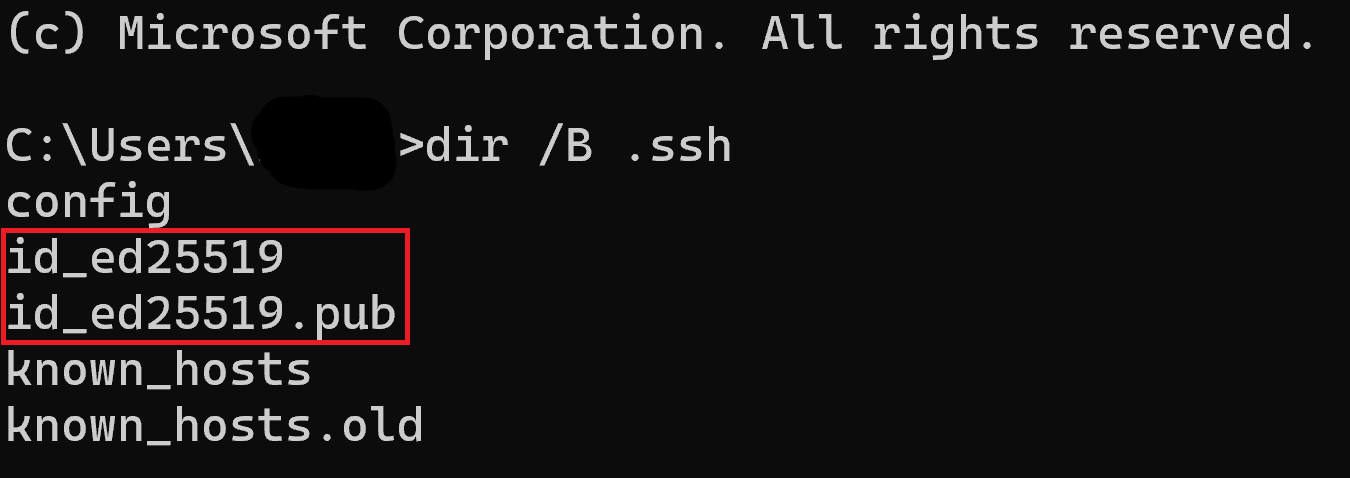
\includegraphics[width=0.7\textwidth]{existing_ssh_keys.png}
        \caption{Existing SSH Keys in \texttt{\mytexttilde/.ssh} Directory}
        \label{fig:existing_ssh_keys}
    \end{figure}
\end{enumerate}

\subsection{Generating the SSH Key}
\begin{enumerate}
    \setcounter{enumi}{3}
    \item Generate an ED25519 SSH key by typing the following command:
    \begin{lstlisting}[style=custombash]
ssh-keygen -t ed25519
    \end{lstlisting}
    \item When prompted for a file in which to save the key, press \textbf{Enter} to accept the default location or specify a custom path.
    \item If prompted to overwrite an existing key, choose to proceed or specify a different filename.
    \item When prompted for a passphrase, you can press \textbf{Enter} to leave it empty or enter a secure passphrase (recommended if using an SSH agent).

    \begin{figure}[H]
        \centering
        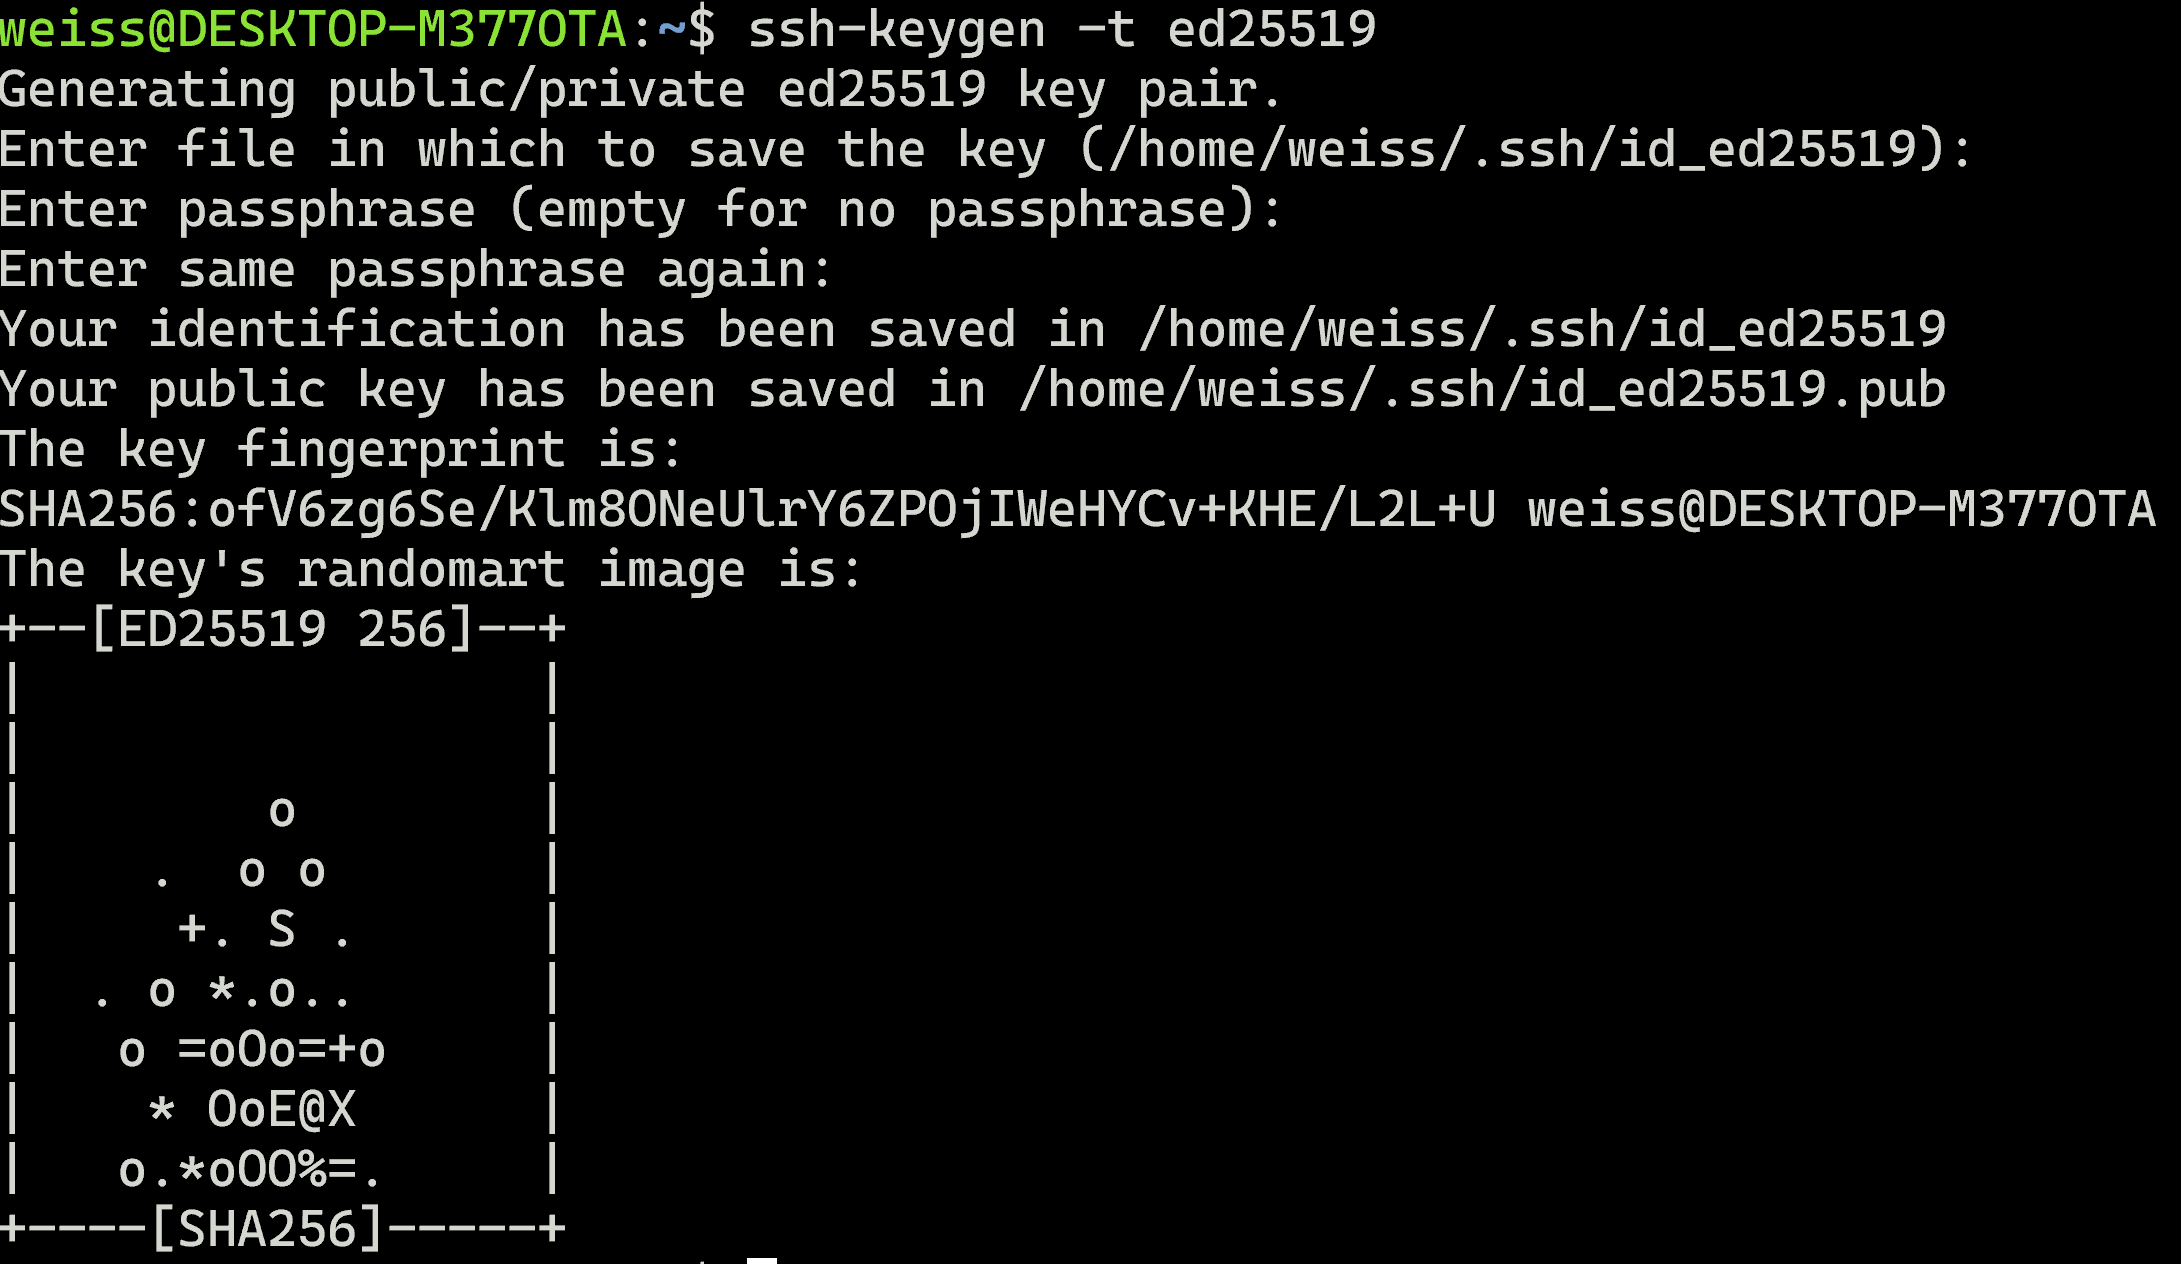
\includegraphics[width=0.7\textwidth]{ssh_keygen.png}
        \caption{Generating SSH Key}
        \label{fig:ssh_keygen}
    \end{figure}
\end{enumerate}

\section{Adding the SSH Key to the SSH Agent}

An SSH agent holds your private keys in memory, allowing you to use them without re-entering your passphrase every time. Follow the instructions for your operating system.

\subsection{macOS and Linux}

\begin{enumerate}
    \item Start the SSH agent:
    \begin{lstlisting}[style=custombash]
eval "$(ssh-agent -s)"
    \end{lstlisting}
    \item Add your private key to the SSH agent:
    \begin{lstlisting}[style=custombash]
ssh-add ~/.ssh/id_ed25519
    \end{lstlisting}
    \item If prompted, enter your passphrase.
    \item Verify that your key has been added:
    \begin{lstlisting}[style=custombash]
ssh-add -l
    \end{lstlisting}
    \item You should see a list of your added SSH keys.
\end{enumerate}

\subsection{Windows (Using OpenSSH Agent)}

\begin{enumerate}
    \item Ensure the SSH agent service is running and set to start automatically. Run the following command in \textbf{PowerShell} as Administrator:
    \begin{lstlisting}[style=custombash]
Get-Service ssh-agent | Set-Service -StartupType Automatic -PassThru | Start-Service
    \end{lstlisting}
    \item Add your private key to the SSH agent. Run the following commands again in the \textbf{Command Prompt}:
    \begin{lstlisting}[style=custombash]
ssh-add %USERPROFILE%\.ssh\id_ed25519
    \end{lstlisting}
    \item If prompted, enter your passphrase.
    \item Verify that your key has been added:
    \begin{lstlisting}[style=custombash]
ssh-add -l
    \end{lstlisting}
    \item You should see a list of your added SSH keys.
\end{enumerate}

\textbf{Note:} If you're using PuTTY's Pageant as your SSH agent:

\begin{enumerate}
    \item Open Pageant.
    \item Click on \textbf{Add Key}.
    \item Navigate to your private key file. If your key is in OpenSSH format, you may need to convert it using PuTTYgen.
    \item Enter your passphrase if prompted.
    \item The key is now loaded into Pageant.
\end{enumerate}

\section{Copying the Public Key to the Server}
Depending on your operating system, follow the appropriate method to copy the public key to the server:

    \subsection{For macOS/Linux Users: Using ssh-copy-id}

    \begin{enumerate}
        \item Use the \texttt{ssh-copy-id} command to copy your public key to the server. Replace \texttt{your\_netid} with your actual NetID:
        \begin{lstlisting}[style=custombash]
ssh-copy-id your_netid@ganymede2.circ.utdallas.edu
        \end{lstlisting}
        \item When prompted, type \texttt{yes} to continue connecting and press \textbf{Enter}.
        \item Enter your \textbf{NetID password} when prompted.
        \item This command appends your public key to the \texttt{authorized\_keys} file on the server automatically.
    \end{enumerate}

    \begin{figure}[H]
        \centering
        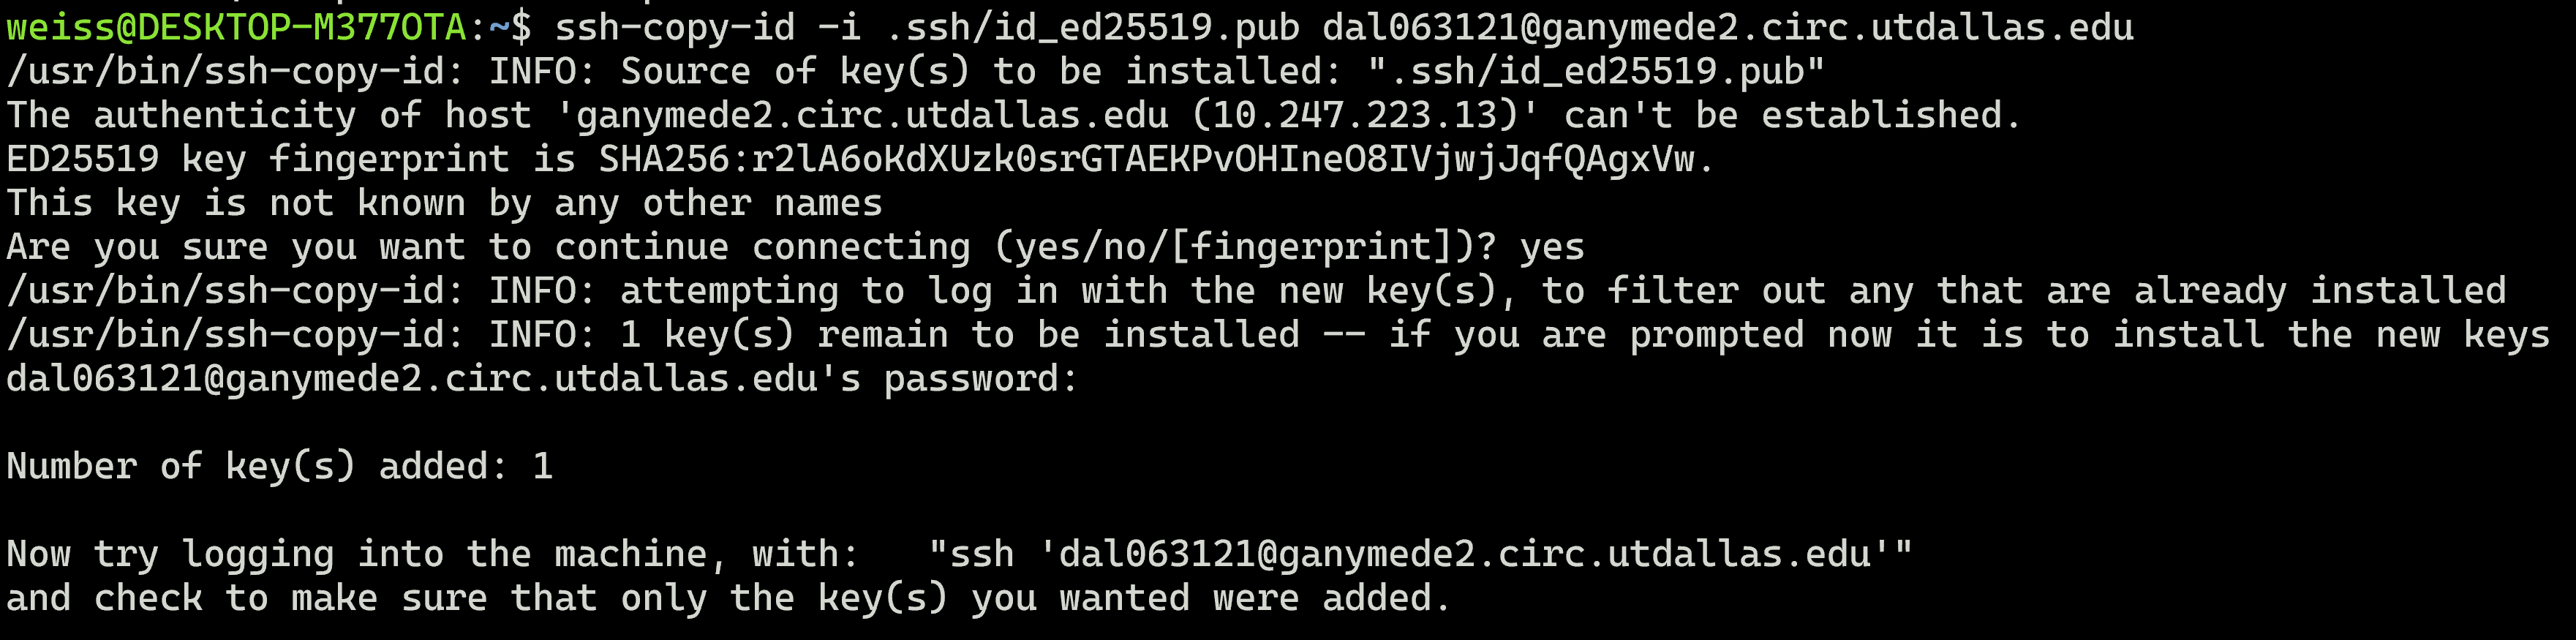
\includegraphics[width=0.7\textwidth]{ssh_copy_id.png}
        \caption{Using ssh-copy-id to Copy Public Key}
        \label{fig:ssh_copy_id}
    \end{figure}

    \subsection{For Windows Users: Command-Line Method}

    \begin{enumerate}
        \item Open \textbf{Command Prompt}.
        \item Use the following command to copy your public key to the server. Replace \texttt{your\_netid} with your actual NetID:
        \begin{lstlisting}[style=custombash]
type %USERPROFILE%\.ssh\id_ed25519.pub | ssh your_netid@ganymede2.circ.utdallas.edu "cat >> /home/your_netid/.ssh/authorized_keys"
        \end{lstlisting}
        \item When prompted, enter your \textbf{NetID password}.
        \item This command appends your public key to the \texttt{authorized\_keys} file on the server automatically.
    \end{enumerate}

    \subsection{Alternative Method for Windows and Other Systems: Manual Copy via Browser}

    If the command-line method doesn't work, you can manually copy your public key to the server:

    \begin{enumerate}
        \item Locate your public key file, typically found at \texttt{\mytexttilde/.ssh/id\_ed25519.pub}.
        \item Open the file (\texttt{id\_ed25519.pub}) and copy the entire contents. \textbf{Never share your private key!}
        \item Open a web browser and navigate to \url{https://g2-ood.circ.utdallas.edu}.
        \item Log in with your credentials.
        \item Click on \textbf{Files} and \textbf{Home Directory}, then check the \textbf{Show dot files} box.
        \item Navigate to your \texttt{\mytexttilde/.ssh} directory. (If it doesn't exist, create it.)
        \item Open the \texttt{authorized\_keys} file (or create it if it doesn't exist).
        \item Paste your \textbf{public key} on a \textbf{new line} in the file and \textbf{save} it.
    \end{enumerate}

    \begin{figure}[H]
        \centering
        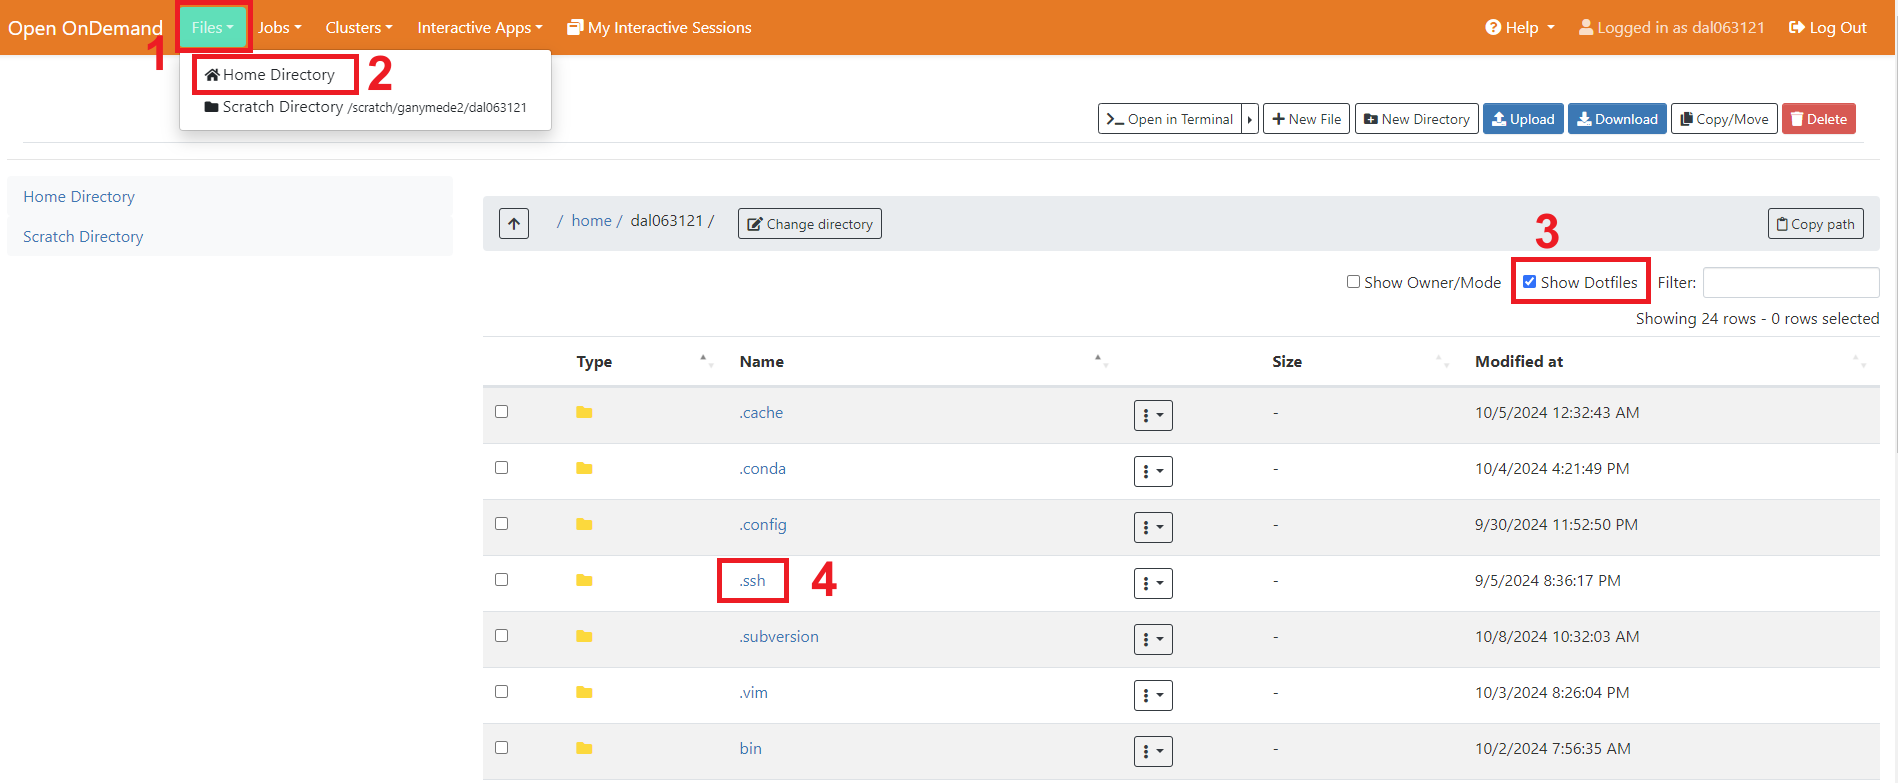
\includegraphics[width=0.7\textwidth]{authorized_keys.png}
        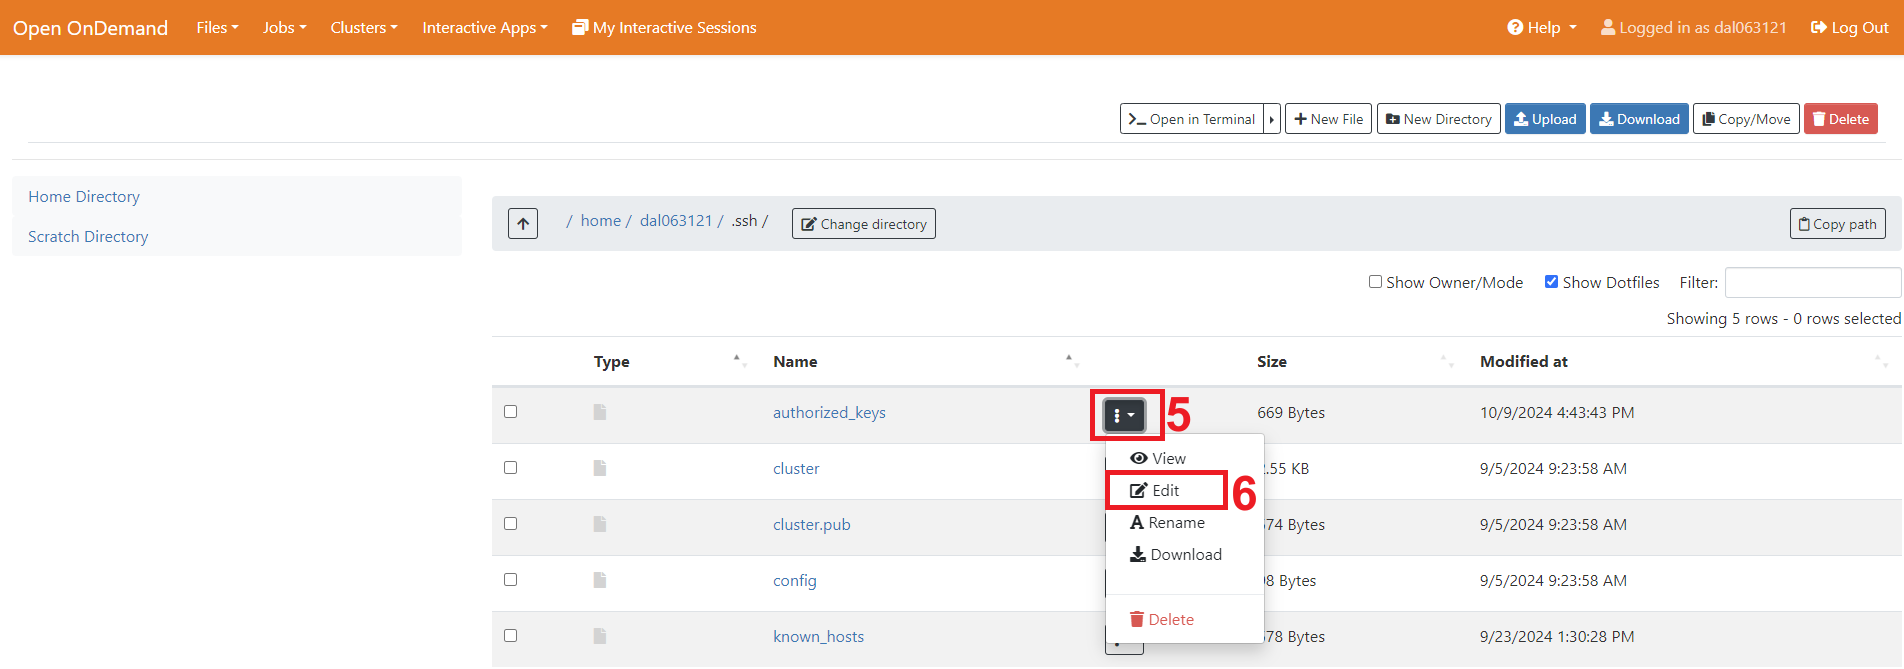
\includegraphics[width=0.7\textwidth]{authorized_keys2.png}
        \caption{Pasting Public Key into \texttt{authorized\_keys}}
        \label{fig:authorized_keys}
    \end{figure}

\section{Conclusion}

You have successfully generated an SSH key pair, added your private key to the SSH agent, and uploaded your public key to the cluster. This will enable secure, password-less authentication when connecting to the server.

\end{document}

